% DESENVOLVIMENTO DA APLICAÇÃO-------------------------------------------------------------------

\chapter{DESENVOLVIMENTO DA APLICAÇÃO}
A proposta para este trabalho foi a construção de uma aplicação que ficaria responsável
por aguardar e coletar as coordenadas geográficas dos pedidos gerados no estabelecimento,
juntamente com o desenvolvimento de um servidor encarregado de gerenciar os pedidos como entregas
com um painel de controle para geração de lotes de entregas e o desenvolvimento de um módulo destinado ao motoboy, no qual consegue observar, em um mapa, a posição e pontos de parada que devem ser percorridos no lote disponível para entrega, tudo isso em tempo real.

\section{Softwares utilizados}

Esta Seção apresenta os \textit{Softwares} utilizados na etapa de codificação da aplicação.

\begin{itemize}
%%% Original: \item PhpStorm: editor de textos que pode ser usado no desenvolvimento de projetos e diversas linguagem de programação;
    \item PhpStorm: IDE completa de desenvolvimento para projetos codificados com a linguagem de programação PHP;
    \item Composer: gerenciador de pacotes em nível de aplicativo, que fornece um formato padrão para gerenciar dependências de software PHP e bibliotecas necessárias;
%%% Original: \item Cmder: “terminal” para o Windows, com essa ferramenta é possível rodar comandos UNIX (\textit{ls}, \textit{rm}, \textit{mv} e etc) diretamente no Windows;
    \item Cmder: console para execução de linhas de comandos para o sistema operacional Windows, com essa ferramenta é possível executar comandos UNIX (\textit{ls}, \textit{rm}, \textit{mv} e etc) diretamente no Windows;
    \item Laravel: \textit{framework} de programação baseada na linguagem PHP;
    \item Artisan CLI: interface de linha de comando incluída no Laravel, fornecendo vários comandos úteis durante a criação da aplicação, por exemplo: configuração de ambiente, verificar rotas, interagir com a aplicação e criar diversos tipos de arquivos (\textit{Migrations}, \textit{Controllers} e \textit{Models});
%%% Original: \item Blade: criação de interface gráfica o Laravel utiliza uma ferramenta de \textit{template}, trazendo uma quantidade grande de ferramentas que ajudam na criação de bonitas interfaces de forma rápida;
    \item Blade: ferramenta para criação de interface gráfica, utilizado pelo Laravel como uma ferramenta de \textit{template}, trazendo uma quantidade grande de funcionalidades que ajudam na criação de interfaces interativas;
    \item Eloquent ORM: ferramenta com funcionalidades que facilitam a inserção, atualização, busca e exclusão de registros diretamente no banco de dados;
    \item XAMPP: servidor independente de plataforma, que consiste principalmente na base de dados MySQL, o servidor web Apache e os interpretadores para linguagens de \textit{script}: PHP e Perl;
    \item Jaspersoft Studio: ferramenta para projetar e executar modelos de relatório com  expressões, gráficos, mapas, tabelas e \textit{QR Codes}, criando documentos de qualquer complexidade a partir de informações presentes no banco de dados;
    \item Sourcetree: representação visual de repositórios da nuvem;
    \item GitHub: plataforma de hospedagem de código-fonte com controle de versão.
\end{itemize}

\section{Coleta de dados}

%%% Rev-Madalozzo: Aqui no módulo de gerenciamento sugiro você listar todos os pacotes de terceiros que é util e que você utilizou na tua aplicação. Por exemplo, na aula usamos o AdminLTE, caso tu uso algum módulo de terceiros lista neste Capítulo

\section{Módulo de gerenciamento}
Ao utilizar o comando \textit{composer create-project --prefer-dist laravel/laravel delivery-routes} no Cmder, dentro de uma pasta no sistema operacional destinada a programação da aplicação, foi criada a estrutura base do projeto, cedida pelo Laravel, apresentada na \autoref{fig:base-projeto}. A facilidade na criação do projeto se deve ao Cmder, que torna o trabalho no sistema operacional da Microsoft mais agradável, com essa ferramenta é possível rodar comandos do Linux e MAC que são baseados em UNIX para o Windows. Embora nas versões mais recentes do Windows (>= 8.1) já tenha o \textit{Power Shell} que atende bem a maiorias de comandos UNIX (que são essenciais para desenvolvedores) ainda sim é totalmente recomendado utilizar alguma ferramenta que nivela estes pontos.

\begin{figure}[H]
    \centering
    \caption{Estrutura Laravel}
    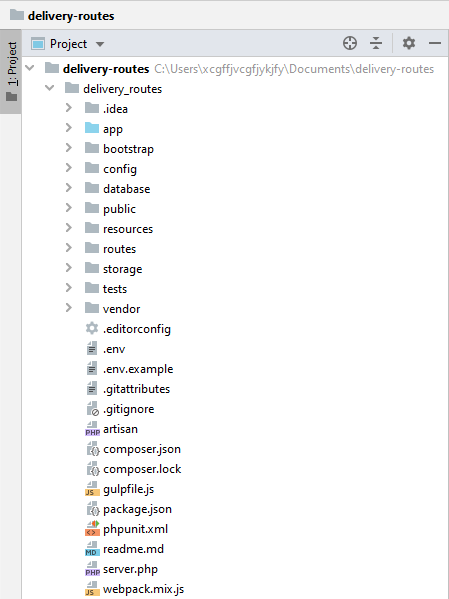
\includegraphics[width=0.6\textwidth]{./dados/figuras/fig6}
    \fonte{Autor}
    \label{fig:base-projeto}
\end{figure}

\begin{figure}[H]
    \centering
    \caption{Delivery Routes - Página inicial}
    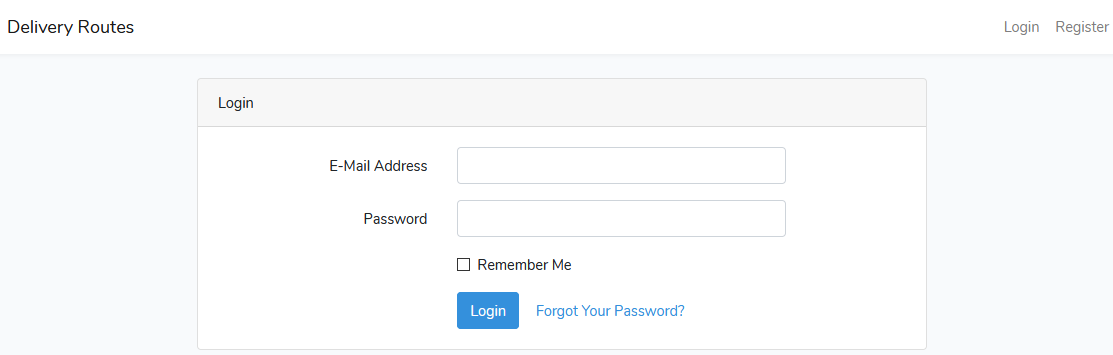
\includegraphics[width=0.9\textwidth]{./dados/figuras/fig7}
    \fonte{Autor}
    \label{fig:apphome}
\end{figure}

\subsection{Painel de gerenciamento}

\section{Consulta de dados}

\section{Módulo de entrega}